\section{Experimental Results \& Tests}
Using our implementation, TRE and scan\_for\_matches, we were able to do some benchmarking in order to compare performances.

For this a virtual machine is created, using Oracle VirtualBox\footnote{virtualbox.org}. The machine running the virtualbox is running Windows 8.1 Pro x64 on an SSD, with 8,00 GB RAM, an AMD FX 4300 Quad-Core Processor 3.80 GHz, of which 1 core and 4096MB RAM was given to the virtual machine, which would run Ubuntu 14.04.2 LTS 64 bit.

\begin{wrapfigure}{r}{0.5\linewidth}
\centering
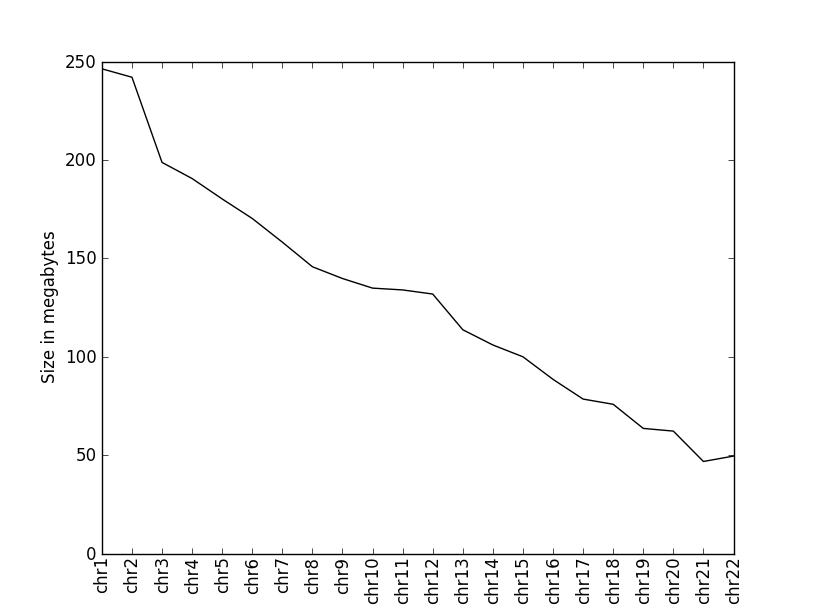
\includegraphics[width=0.3\textwidth]{Benchmarking/size.png}
\caption{Plot of sample files used for benchmarking, these files range from 246.3 Megabytes to 46.8 Megabytes in size}
\label{fig:size}
\end{wrapfigure}

For the benchmarking some data was required. Figure~\ref{fig:size} shows a series of fasta files, and these files include nucleotide sequences, which all differ in size, decreasing from chr1 to chr22. These fasta files are the  kind of data which scan\_for\_matches is expected to run, and thus excellent for benchmark testing. It is worth noting however, that each of these files' lines are 50 characters long, and as TRE matches through lines separately, and longer or shorter line sizes might affect the performance of TRE. This was not tested however.

For testing, a suitable pattern is required. As our implementation has primarily been focused on supporting insertion, deletion and mutation on a sequence, a simple RNA sequence $TGCAAGCGTTAAT$ with variable insertions is chosen as the search pattern.

Each test would be executed on each of the mentioned fasta files a total of 10 times, given an average runtime which was used in the following results.

\begin{figure}[h!]
\centering
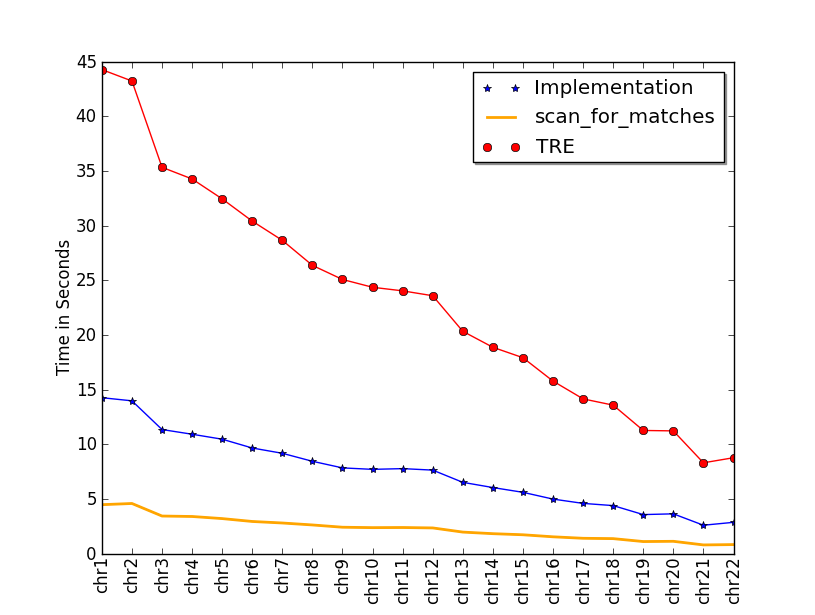
\includegraphics[width=0.5\textwidth]{Benchmarking/0miss.png}
\caption{Running time of search through fasta files mentioned in figure~\ref{fig:size} looking for pattern TGCAAGCGTTAAT with no mismatches}
\label{fig:0miss}
\end{figure}

First test was to see the runtime of each program, having no mismatches in the mentioned sequence $TGCAAGCGTTAAT$. Figure~\ref{fig:0miss} displays the results, and it is clear to see that scan\_for\_matches is faster than both our implementation and TRE, and that all three programs have a decreased runtime as the data sizes lowers.

\begin{figure}[h!]
\begin{minipage}[b]{0.5\linewidth}
\centering
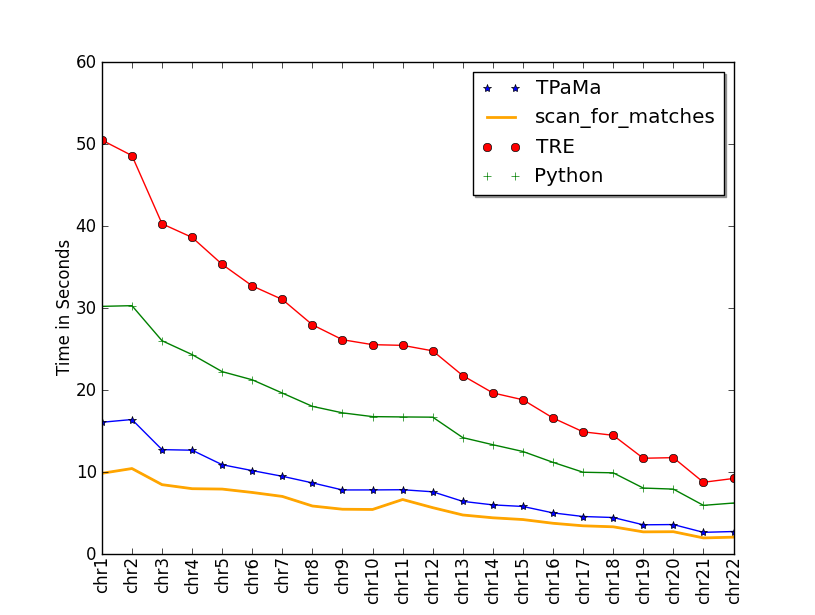
\includegraphics[width=0.8\textwidth]{Benchmarking/1ins.png}
\caption{Running time of search through fasta files mentioned in figure~\ref{fig:size},  allowing one insertions on pattern TGCAAGCGTTAAT}
\label{fig:ins1}
\end{minipage}
\hspace{0.25cm}
\begin{minipage}[b]{0.5\linewidth}
\centering
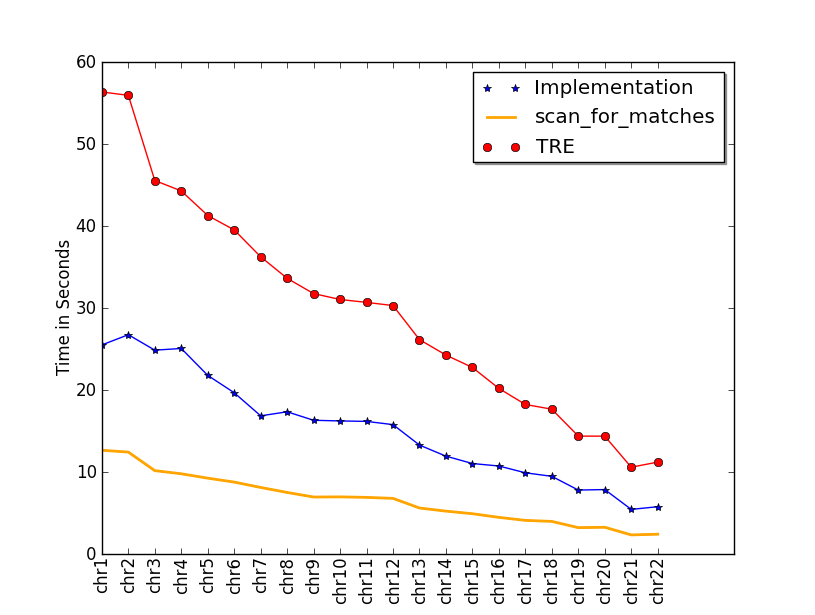
\includegraphics[width=0.8\textwidth]{Benchmarking/2ins.png}
\caption{Running time of search through fasta files mentioned in figure~\ref{fig:size},  allowing two insertions on pattern TGCAAGCGTTAAT}
\label{fig:ins2}
\end{minipage}
\end{figure}


From figure~\ref{fig:ins1} it is clear that there is an increase in the runtime for our implementation when adding an insertion to its pattern, and while both our scan\_for\_matches and TRE also has an increased runtime, it is not to the same scale as our implementation.

Next test was to see the runtime of two insertions instead of one. Looking at figure~\ref{fig:ins2}, scan\_for\_matches did increase its runtime slightly compared to figure~\ref{fig:ins1}, but the second insertion greatly affected our implementation, resulting in it running at about half the speed of TRE.  And while TRE also had its runtime slightly increased, it's almost unchanged from one insertion.

\begin{figure}[h!]
\centering
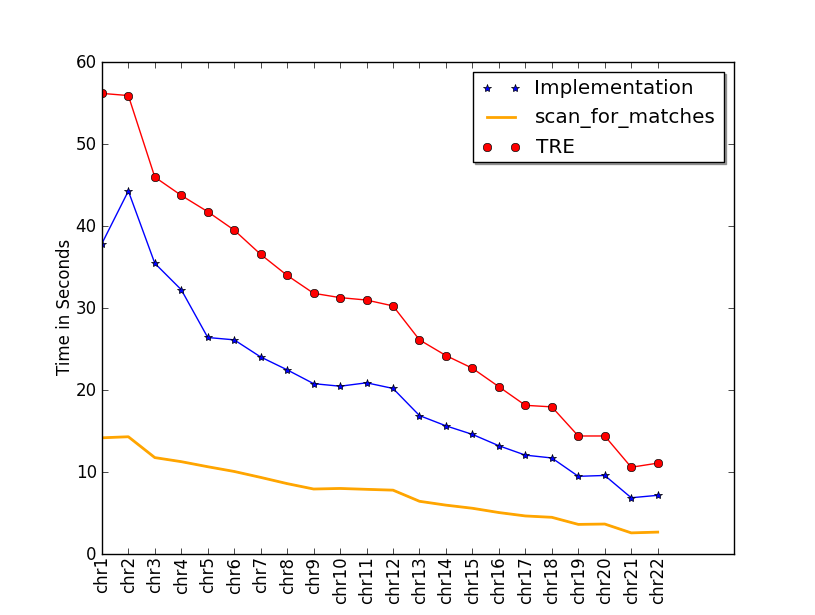
\includegraphics[width=0.5\textwidth]{Benchmarking/3ins.png}
\caption{Running time of search through fasta files mentioned in figure~\ref{fig:size},  allowing three insertions on pattern TGCAAGCGTTAAT}
\label{fig:ins3}
\end{figure}
Testing with three insertions, figure~\ref{fig:ins3} shows that once again our implementation had the worst increase in time compared to the two other options, almost reaching the same runtime as TRE.


From these three tests its clear to see that our implementation has a problem with increasing number of insertions, increasing its runtime at a much higher rate than both scan\_for\_matches and TRE. From this we can conclude that our current implementation has a major flaw somewhere, should it be used with more advanced patterns. 
\\
~

Another interesting thing to test for was the number of hits when searching the files, in table~\ref{tab:hits} the number of hits which came up when searching on file chr1.fa are shown.

\begin{table}[h!]
\centering
\begin{tabular}{ l | c c r }
& 1 insertion & 2 insertions & 3 insertions\\
\hline
Our implementation& 5 &  47 & 235 \\
TRE& 1 & 19 & 76 \\
scan\_for\_matches & 5 & 43  & 192 \\
\end{tabular}
\caption{Number of hits in fasta file chr1, using the mentioned benchmark tests.}
\label{tab:hits}
\end{table}

The primary reason that our implementation gets more results than scan\_for\_matches is that our implementation finds every single match in the file, including overlapping matches, while scan\_for\_matches, by default, only finds matches which does not overlap. TRE has the major disadvantage here that it doesn't match across newlines, causing it to miss a lot of matches.

